\documentclass[12pt]{report}
\usepackage{tikz}
\usepackage{parskip}
\usepackage{mathtools}
\usepackage{flexisym}



\begin{document}
\newcommand\tab[1][1cm]{\hspace*{#1}}

%title page
\author{Andre Gregoire}
\title{CIS770 Homework 4}
\maketitle

%problem 1
\textbf{ Problem1}\newline
\textit{1.1.}\newline
\begin{flushleft}
I first converted the Language L = \textbf{L}(1\textsuperscript{*}0(00$\cup$01$\cup$1)(0$\cup$1)\textsuperscript{*}) into a DFA M: \newline
\begin{center}
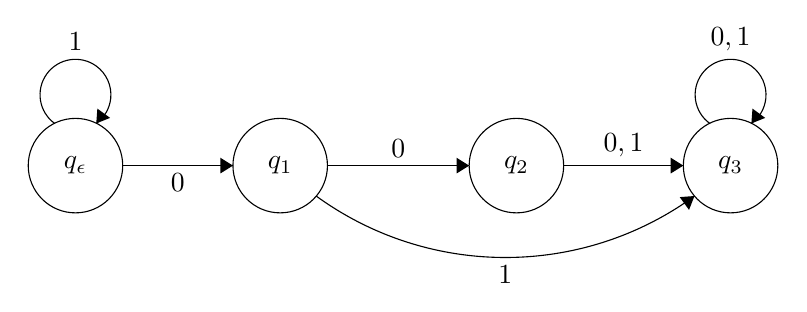
\begin{tikzpicture}[scale=0.2]
\tikzstyle{every node}+=[inner sep=0pt]
\draw [black] (9.1,-19.8) circle (3);
\draw (9.1,-19.8) node {$q_\epsilon$};
\draw [black] (22.1,-19.8) circle (3);
\draw (22.1,-19.8) node {$q_1$};
\draw [black] (37.1,-19.8) circle (3);
\draw (37.1,-19.8) node {$q_2$};
\draw [black] (50.7,-19.8) circle (3);
\draw (50.7,-19.8) node {$q_3$};
\draw [black] (7.777,-17.12) arc (234:-54:2.25);
\draw (9.1,-12.55) node [above] {$1$};
\fill [black] (10.42,-17.12) -- (11.3,-16.77) -- (10.49,-16.18);
\draw [black] (12.1,-19.8) -- (19.1,-19.8);
\fill [black] (19.1,-19.8) -- (18.3,-19.3) -- (18.3,-20.3);
\draw (15.6,-20.3) node [below] {$0$};
\draw [black] (25.1,-19.8) -- (34.1,-19.8);
\fill [black] (34.1,-19.8) -- (33.3,-19.3) -- (33.3,-20.3);
\draw (29.6,-19.3) node [above] {$0$};
\draw [black] (40.1,-19.8) -- (47.7,-19.8);
\fill [black] (47.7,-19.8) -- (46.9,-19.3) -- (46.9,-20.3);
\draw (43.9,-19.3) node [above] {$0,1$};
\draw [black] (48.41,-21.734) arc (-54.01274:-125.98726:20.44);
\fill [black] (48.41,-21.73) -- (47.47,-21.8) -- (48.06,-22.61);
\draw (36.4,-26.14) node [below] {$1$};
\draw [black] (49.377,-17.12) arc (234:-54:2.25);
\draw (50.7,-12.55) node [above] {$0,1$};
\fill [black] (52.02,-17.12) -- (52.9,-16.77) -- (52.09,-16.18);
\end{tikzpicture}
\end{center}

Now we can list the suffix language for each state in M.\newline
\tab $q_\epsilon$ = L\newline
\tab $q_1$ = (00 $\cup$ 01 $\cup$ 1)(0$\cup$1)\textsuperscript{*}\newline
\tab $q_2$ = (0 $\cup$ 1)(0 $\cup$ 1)\textsuperscript{*}\newline
\tab $q_3$ = (0 $\cup$ 1)\textsuperscript{*}\newline

Because M is a DFA that accepts L, the suffix languages derived from M cover all suffix languages in the language L.\newline
\end{flushleft}


\textit{1.2.}\newline
\begin{flushleft}
The DFA M used to come up with solution to \textit{problem 1.1} is the minimal state DFA M\textsuperscript{L} accepting L: 
\begin{center}
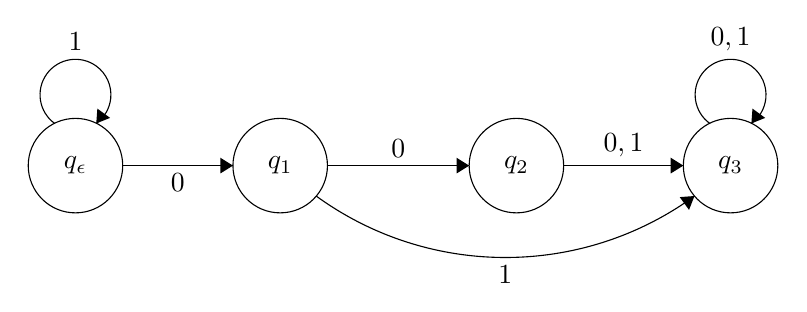
\begin{tikzpicture}[scale=0.2]
\tikzstyle{every node}+=[inner sep=0pt]
\draw [black] (9.1,-19.8) circle (3);
\draw (9.1,-19.8) node {$q_\epsilon$};
\draw [black] (22.1,-19.8) circle (3);
\draw (22.1,-19.8) node {$q_1$};
\draw [black] (37.1,-19.8) circle (3);
\draw (37.1,-19.8) node {$q_2$};
\draw [black] (50.7,-19.8) circle (3);
\draw (50.7,-19.8) node {$q_3$};
\draw [black] (7.777,-17.12) arc (234:-54:2.25);
\draw (9.1,-12.55) node [above] {$1$};
\fill [black] (10.42,-17.12) -- (11.3,-16.77) -- (10.49,-16.18);
\draw [black] (12.1,-19.8) -- (19.1,-19.8);
\fill [black] (19.1,-19.8) -- (18.3,-19.3) -- (18.3,-20.3);
\draw (15.6,-20.3) node [below] {$0$};
\draw [black] (25.1,-19.8) -- (34.1,-19.8);
\fill [black] (34.1,-19.8) -- (33.3,-19.3) -- (33.3,-20.3);
\draw (29.6,-19.3) node [above] {$0$};
\draw [black] (40.1,-19.8) -- (47.7,-19.8);
\fill [black] (47.7,-19.8) -- (46.9,-19.3) -- (46.9,-20.3);
\draw (43.9,-19.3) node [above] {$0,1$};
\draw [black] (48.41,-21.734) arc (-54.01274:-125.98726:20.44);
\fill [black] (48.41,-21.73) -- (47.47,-21.8) -- (48.06,-22.61);
\draw (36.4,-26.14) node [below] {$1$};
\draw [black] (49.377,-17.12) arc (234:-54:2.25);
\draw (50.7,-12.55) node [above] {$0,1$};
\fill [black] (52.02,-17.12) -- (52.9,-16.77) -- (52.09,-16.18);
\end{tikzpicture}
\end{center}
\end{flushleft}
\pagebreak
%problem 2
\textbf{Problem 2}\newline
\textit{2.1.}
\begin{flushleft}
By the definition of Homomorphism discussed in class \\
A Homomorphism is a function h : $\Sigma\textsuperscript{*} \rightarrow \Delta\textsuperscript{*}$ defined as: \\
\tab h($\epsilon$) = $\epsilon$ and for a $\in$ $\Sigma$, h(a) is any string in $\Delta$\textsuperscript{*} \\
\tab For a = $a_1a_2..a_n$ $\in$ $\Sigma$\textsuperscript{*} (n $\geq$ 2), h(a) = h($a_1$)h($a_2$)...h($a_n$).\newline

By using the second axiom from our definition:\\
\tab a = xy \\
\tab $a_1$ = x, $a_2$ = y and n = 2 \\
\tab we can see that h(a) = h($a_1$)h($a_2$) = h(x)h(y)
\end{flushleft}

\textit{2.2.}
\begin{flushleft}
h($L_1 \cup L_2$) = h($L_1$) $\cup$ h($L_2$)\\
h($L_1 \cup L_2$) = \{ h(\textit{w}) $\vert$ \textit{w} $\in$ $L_1 \cup L_2$\}\\
Let \textit{w} $\in$ h($L_1 \cup L_2$) \\
\tab $\Rightarrow$ $\exists$ \textit{u}. \textit{u} $\in$ $L_1 \cup L_2$ and \textit{w} = h(\textit{u})\\
\tab $\Rightarrow$ $\exists$ \textit{u}. \textit{u} $\in$ $L_2$ and \textit{w} = h(\textit{u})\\
\tab $\Rightarrow$ \textit{w} $\in$ h($L_2$)\\
\tab $\Rightarrow$ \textit{w} $\in$ h($L_1$)  $\cup$ h($L_2$)\\
\end{flushleft}


\textit{2.3.}
\begin{flushleft}
h($L_1 \circ L_2$) = h($L_1$) $\circ$ h($L_2$)\\
h($L_1 \circ L_2$) = \{ h(\textit{w}) $\vert$ \textit{w} $\in$ $L_1 \circ L_2$\}\\
Let \textit{w} $\in$ h($L_1 \circ L_2$) 
 $\Rightarrow$ $\exists$ \textit{u}. \textit{u} $\in$ $L_1 \circ L_2$ and \textit{w} = h(\textit{u})\\
Let \textit{a} $\in$ h($L_1$) 
 $\Rightarrow$ $\exists$ \textit{x}. \textit{x} $\in$ $L_1$ and \textit{a} = h(\textit{x})\\
Let \textit{b} $\in$ h($L_1$) 
 $\Rightarrow$ $\exists$ \textit{y}. \textit{y} $\in$ $L_1$ and \textit{b} = h(\textit{y})\\
\tab $\Rightarrow$ \textit{u} = \textit{x} $\circ$ \textit{y}\\
\tab $\Rightarrow$ \textit{w} = \textit{a} $\circ$ \textit{b}\\
\tab $\Rightarrow$ \textit{w} $\in$ h($L_1$) $\circ$ h($L_2$)\\


\end{flushleft}


\end{document}
